\documentclass[11pt]{article}

\usepackage[T1]{fontenc}
\usepackage[utf8]{inputenc}
\usepackage[french]{babel}
\usepackage{amsmath, amssymb, amsthm}
\usepackage{graphicx}
\usepackage{geometry}
\usepackage{enumitem}
\usepackage{hyperref}
\usepackage{mdframed}
\usepackage{mathtools}

\geometry{margin=2.5cm}

% --- Macros utiles ---
\newcommand{\RR}{\mathbb{R}}
\newcommand{\oo}{+\infty}
\newcommand{\fonction}[5]{#1 : #2 \to #3,\quad #4 \mapsto #5}
\newcommand{\acompleter}{\fbox{À compléter}}
\newcommand{\calC}{\mathcal{C}}

% --- Style des cadres ---
\mdfdefinestyle{coursbox}{
  linewidth=0.8pt,
  linecolor=black,
  backgroundcolor=white,
  roundcorner=0pt,
  innertopmargin=8pt,
  innerbottommargin=8pt,
  innerleftmargin=10pt,
  innerrightmargin=10pt,
  skipabove=10pt,
  skipbelow=10pt
}

% --- Environnements simples ---
\newenvironment{remarque}{\par\smallskip\noindent\textbf{Remarque. \\}\ignorespaces}{\par\smallskip}
\newenvironment{exemple}{\par\smallskip\noindent\textbf{Exemple. \\}\ignorespaces}{\par\smallskip}
\newenvironment{demonstration}{\par\smallskip\noindent\textbf{Démonstration. \\}\ignorespaces}{\par\smallskip}
\newenvironment{exemples}{\par\smallskip\noindent\textbf{Exemples. \\}\ignorespaces}{\par\smallskip}

% --- Environnements encadrés ---
\newmdenv[style=coursbox]{definition}
\newmdenv[style=coursbox]{propriete}
\newmdenv[style=coursbox]{definitions}

\begin{document}

\begin{definition}
\begin{center}
    {\Huge\bfseries Second degré - 2/2}
\end{center}
\end{definition}

\begin{remarque}
Les méthodes de résolution des équations du second degré se sont développées progressivement. Les Babyloniens résolvaient déjà certains cas particuliers vers 2000 avant J.-C. ; au VII\textsuperscript{e} siècle, le mathématicien indien Brahmagupta formula des règles générales. Au IX\textsuperscript{e} siècle, Al-Khawarizmi systématisa ces méthodes dans son traité d'algèbre.

La notion de discriminant fut introduite par les mathématiciens européens de la Renaissance, notamment François Viète (1540--1603), qui établit des relations entre les coefficients et les racines. L'étude moderne des équations et des inéquations du second degré fut ensuite développée, entre autres, par René Descartes et Leonhard Euler.
\end{remarque}

\section{Résolution d'une équation du second degré}

\begin{definition}
Soit une équation du second degré de la forme
\[
ax^2+bx+c=0,
\]
où $a$, $b$ et $c$ sont des réels tels que $a\neq 0$.

Une solution de cette équation s'appelle une \emph{racine} du trinôme $ax^2+bx+c$.
\end{definition}

\begin{exemple}
$3x^2-5x-2=0$ est une équation du second degré. Le nombre $2$ en est une racine, car
\[
3\times 2^2-5\times 2-2=0.
\]
\end{exemple}

\begin{definition}
On appelle \emph{discriminant} du trinôme $ax^2+bx+c$ le nombre réel, noté $\Delta$, défini par
\[
\Delta=b^2-4ac.
\]
\end{definition}

\begin{propriete}
\textbf{Propriété}\\
Soit $\Delta$ le discriminant du trinôme $ax^2+bx+c$.
\begin{itemize}
    \item Si $\Delta>0$, l'équation a deux solutions distinctes :
    \[
    x_1=\frac{-b-\sqrt{\Delta}}{2a}
    \qquad\text{et}\qquad
    x_2=\frac{-b+\sqrt{\Delta}}{2a}.
    \]
    Le trinôme admet alors deux racines réelles.
    \item Si $\Delta=0$, l'équation a une unique solution :
    \[
    x_0=-\frac{b}{2a}.
    \]
    Le trinôme admet alors une racine double.
    \item Si $\Delta<0$, l'équation n'a pas de solution réelle et le trinôme n'a pas de racine réelle.
\end{itemize}
\end{propriete}

\begin{exemples}
Résoudre les équations suivantes dans $\RR$ :
\begin{enumerate}[label=\arabic*.]
    \item $x^2+3x-10=0$ ;
    \item $3x^2+2x+2=0$ ;
    \item $18x^2-12x+2=0$.
\end{enumerate}

\begin{enumerate}[label=\arabic*.]
    \item Le discriminant de $x^2+3x-10$ est
    \[
    \Delta=3^2-4\times1\times(-10)=49.
    \]
    Comme $\Delta>0$, l'équation a deux solutions :
    \[
    x_1=\frac{-3-\sqrt{49}}{2\times1}=-5
    \qquad\text{et}\qquad
    x_2=\frac{-3+\sqrt{49}}{2\times1}=2.
    \]
    L'ensemble des solutions est donc $\{-5\,;\,2\}$.

    \item Le discriminant de $3x^2+2x+2$ est
    \[
    \Delta=2^2-4\times3\times2=-20.
    \]
    Comme $\Delta<0$, l'équation n'a pas de solution réelle.

    \item Le discriminant de $18x^2-12x+2$ est
    \[
    \Delta=(-12)^2-4\times18\times2=0.
    \]
    L'équation a une unique solution :
    \[
    x_0=-\frac{-12}{2\times18}=\frac{2}{3}.
    \]
\end{enumerate}
\end{exemples}

\begin{demonstration}
On sait que le trinôme peut s'écrire sous forme canonique :
\[
ax^2+bx+c
=a\left(x+\frac{b}{2a}\right)^2-\frac{b^2-4ac}{4a}
=a\left(x+\frac{b}{2a}\right)^2-\frac{\Delta}{4a}.
\]
Ainsi,
\begin{align*}
ax^2+bx+c=0
&\iff a\left(x+\frac{b}{2a}\right)^2-\frac{\Delta}{4a}=0\\
&\iff a\left(x+\frac{b}{2a}\right)^2=\frac{\Delta}{4a}\\
&\iff \left(x+\frac{b}{2a}\right)^2=\frac{\Delta}{4a^2},
\end{align*}
car $a\neq0$.

\begin{itemize}
    \item Si $\Delta<0$, le membre de droite est négatif. Un carré ne pouvant pas être négatif, l'équation n'a pas de solution réelle.
    \item Si $\Delta=0$, on obtient $\left(x+\frac{b}{2a}\right)^2=0$. L'unique solution est $x_0=-\frac{b}{2a}$.
    \item Si $\Delta>0$, on utilise une différence de deux carrés :
    \begin{align*}
    \left(x+\frac{b}{2a}\right)^2
    &=\left(\frac{\sqrt{\Delta}}{2a}\right)^2\\
    \iff\quad
    \left(x+\frac{b}{2a}-\frac{\sqrt{\Delta}}{2a}\right)
    \left(x+\frac{b}{2a}+\frac{\sqrt{\Delta}}{2a}\right)&=0\\
    \iff\quad
    \left(x+\frac{b-\sqrt{\Delta}}{2a}\right)
    \left(x+\frac{b+\sqrt{\Delta}}{2a}\right)&=0.
    \end{align*}
    Les deux solutions sont donc
    \[
    x_1=\frac{-b-\sqrt{\Delta}}{2a}
    \qquad\text{et}\qquad
    x_2=\frac{-b+\sqrt{\Delta}}{2a}.
    \]
\end{itemize}
\end{demonstration}

\section{Factorisation d'un trinôme}

\begin{propriete}
\textbf{Propriété}\\
Soit $f$ une fonction polynôme du second degré définie par $f(x)=ax^2+bx+c$, avec $a\neq0$.
\begin{itemize}
    \item Si $\Delta>0$, alors
    \[
    f(x)=a(x-x_1)(x-x_2),
    \quad\text{où}\quad
    x_1=\frac{-b-\sqrt{\Delta}}{2a}
    \quad\text{et}\quad
    x_2=\frac{-b+\sqrt{\Delta}}{2a}.
    \]
    \item Si $\Delta=0$, alors
    \[
    f(x)=a(x-x_0)^2,
    \quad\text{où}\quad
    x_0=-\frac{b}{2a}.
    \]
    \item Si $\Delta<0$, $f(x)$ n'est pas factorisable en produit de facteurs du premier degré à coefficients réels.
\end{itemize}
\end{propriete}

\begin{exemples}
Factoriser, si possible, les expressions suivantes :
\begin{enumerate}[label=\arabic*.]
    \item $3x^2-x-4$ ;
    \item $3x^2-\dfrac{7}{2}x+\dfrac{49}{48}$ ;
    \item $2x^2+4x+3$.
\end{enumerate}

\begin{enumerate}[label=\arabic*.]
    \item $\Delta=(-1)^2-4\times3\times(-4)=49$. Les racines sont
    \[
    x_1=\frac{1-7}{6}=-1
    \qquad\text{et}\qquad
    x_2=\frac{1+7}{6}=\frac{4}{3}.
    \]
    Ainsi,
    \[
    3x^2-x-4=3(x+1)\left(x-\frac{4}{3}\right)=(x+1)(3x-4).
    \]

    \item
    \[
    \Delta=\left(-\frac{7}{2}\right)^2
    -4\times3\times\frac{49}{48}=0,
    \qquad
    x_0=\frac{7/2}{2\times3}=\frac{7}{12}.
    \]
    Donc
    \[
    3x^2-\frac{7}{2}x+\frac{49}{48}
    =3\left(x-\frac{7}{12}\right)^2.
    \]

    \item $\Delta=4^2-4\times2\times3=-8<0$. L'expression n'est pas factorisable en produit de facteurs du premier degré à coefficients réels.
\end{enumerate}
\end{exemples}

\section{Somme et produit des racines}

\begin{propriete}
\textbf{Propriété}\\
Soit le trinôme $ax^2+bx+c$ ayant deux racines réelles distinctes $x_1$ et $x_2$ (donc $\Delta>0$). Alors
\[
x_1+x_2=-\frac{b}{a}
\qquad\text{et}\qquad
x_1x_2=\frac{c}{a}.
\]
\end{propriete}

\begin{demonstration}
Le trinôme ayant deux racines réelles distinctes, il s'écrit
\begin{align*}
ax^2+bx+c
&=a(x-x_1)(x-x_2)\\
&=a(x^2-xx_2-xx_1+x_1x_2)\\
&=ax^2-a(x_1+x_2)x+ax_1x_2.
\end{align*}
En identifiant les coefficients avec ceux de $ax^2+bx+c$, on obtient
\[
b=-a(x_1+x_2),\qquad c=ax_1x_2,
\]
d'où
\[
x_1+x_2=-\frac{b}{a}
\qquad\text{et}\qquad
x_1x_2=\frac{c}{a}.
\]
\end{demonstration}

\begin{remarque}
On écrit parfois un trinôme sous la forme $a(x^2-Sx+P)$, où $S$ est la somme des racines et $P$ leur produit.
\end{remarque}

\begin{exemple}
Déterminer deux nombres dont la somme vaut $3$ et le produit vaut $-10$.

Ces nombres sont les racines de l'équation $x^2-3x-10=0$. En résolvant cette équation, on trouve $x_1=-2$ et $x_2=5$.
\end{exemple}

\section{Signe du trinôme}

\begin{propriete}
\textbf{Propriété}\\
Soit $f(x)=ax^2+bx+c$ une fonction polynôme du second degré, avec $a\neq0$.
\begin{itemize}
    \item Si $\Delta<0$, le trinôme est du signe de $a$ sur $\RR$ et ne s'annule pas.
    \item Si $\Delta=0$, le trinôme est du signe de $a$ sur $\RR$ et s'annule en son unique racine $x_0$.
    \item Si $\Delta>0$, le trinôme est du signe de $a$ à l'extérieur des racines et du signe de $-a$ entre les racines. Plus précisément, si $x_1<x_2$ sont ses racines, il est :
    \begin{itemize}
        \item du signe de $a$ sur $]-\infty\,;x_1[\cup]x_2\,;+\infty[$ ;
        \item nul en $x_1$ et $x_2$ ;
        \item du signe de $-a$ sur $]x_1\,;x_2[$.
    \end{itemize}
\end{itemize}
\end{propriete}

\begin{remarque}
On retient parfois que \og $f(x)$ est du signe de $a$ en dehors des racines \fg.
\end{remarque}

Si $\Delta>0$ et $x_1<x_2$, le tableau de signes est :
\[
\begin{array}{c|cccccc}
x & -\infty & & x_1 & & x_2 & +\infty\\ \hline
ax^2+bx+c & \text{signe de }a & & 0 & \text{signe de }-a & 0 & \text{signe de }a
\end{array}
\]
Si $\Delta\leq0$, le trinôme est du signe de $a$ sur $\RR$, en tenant compte de son annulation en $x_0$ lorsque $\Delta=0$.

\begin{center}
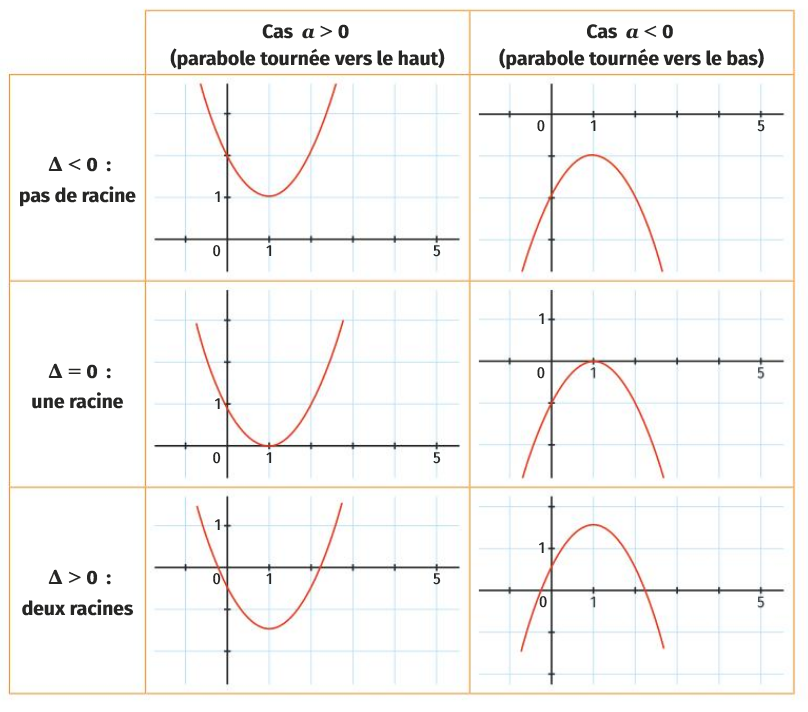
\includegraphics[width=0.65\textwidth]{images/para_sgn.png}
\end{center}

\begin{exemples}
Résoudre dans $\RR$ les inéquations suivantes :
\begin{enumerate}[label=\arabic*.]
    \item $3x^2+5x-2\geq0$ ;
    \item $-x^2+x-7>0$.
\end{enumerate}

\begin{enumerate}[label=\arabic*.]
    \item Les racines de $3x^2+5x-2$ sont $x_1=-2$ et $x_2=\frac{1}{3}$. Comme le coefficient de $x^2$ est positif, le trinôme est positif à l'extérieur des racines et négatif entre elles. Ainsi,
    \[
    3x^2+5x-2\geq0
    \iff x\in]-\infty\,;-2]\cup\left[\frac{1}{3}\,;+\infty\right[.
    \]

    \item Le trinôme $-x^2+x-7$ n'a pas de racine réelle, car son discriminant est négatif. Il est donc toujours du signe de son coefficient de $x^2$, c'est-à-dire négatif. L'inéquation $-x^2+x-7>0$ n'a aucune solution.
\end{enumerate}
\end{exemples}

\section{Application : position relative de deux courbes}

Soient $f$ et $g$ les fonctions définies sur $\RR$ par
\[
f(x)=-x^2+8x-11
\qquad\text{et}\qquad
g(x)=x-1.
\]
Étudions la position relative de leurs courbes représentatives $\calC_f$ et $\calC_g$ en étudiant le signe de $f(x)-g(x)$.

\begin{demonstration}
\[
f(x)-g(x)=-x^2+8x-11-(x-1)=-x^2+7x-10.
\]
Les racines de ce trinôme sont $x_1=2$ et $x_2=5$. Son coefficient de $x^2$ étant négatif, $f(x)-g(x)$ est positif entre les racines et négatif à l'extérieur.

Ainsi, $\calC_f$ est en dessous de $\calC_g$ pour
\[
x\in]-\infty\,;2[\cup]5\,;+\infty[,
\]
et au-dessus de $\calC_g$ pour $x\in]2\,;5[$. Les courbes se coupent pour $x=2$ et $x=5$.
\end{demonstration}

Vérification graphique à l'aide de la calculatrice ou d'un logiciel :
\begin{center}
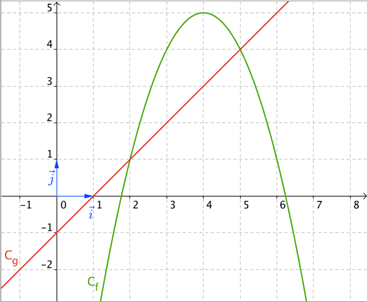
\includegraphics[width=0.5\textwidth]{images/second_degré_1.png}
\end{center}

\end{document}
